% Generated by paper/figures/src/fig_phase2.py baselines; do not edit by hand.
% Generated by fig_phase2.py baselines; frozen selection in gallery_baselines/provenance.json.
% 7961019668960160206: A large gas planet with distinctive rings is depicted, accompanied by a smaller moon and a distant sun glowing in a reddish space background.
% m2679953061215100202: A dancer in mid-pose creates a dynamic splash of water, set against a black background, illuminated to highlight their silhouette.
% m4844341235185759356: A lone hiker stands on a rocky outcrop, overlooking a stunning landscape of dramatic mountains and a serene, reflective body of water at sunset, with vibrant hues of orange, pink, and purple in the sky.
\begin{figure*}[t]
\centering\sffamily\scriptsize\ifdefined\scaW\else\newlength{\scaW}\fi\setlength{\scaW}{\textwidth}
\setlength{\fboxsep}{1pt}\setlength{\lineskip}{0pt}\setlength{\lineskiplimit}{0pt}
\makebox[\textwidth][l]{\makebox[0.1966\scaW][c]{AReA}\hspace{0.0040\scaW}\makebox[0.1966\scaW][c]{DyPE}\hspace{0.0040\scaW}\makebox[0.1966\scaW][c]{SEGA}\hspace{0.0040\scaW}\makebox[0.1966\scaW][c]{UltraImage}\hspace{0.0040\scaW}\makebox[0.1966\scaW][c]{\textbf{SCA (ours)}}}\\[0.0040\textwidth]
\makebox[\textwidth][l]{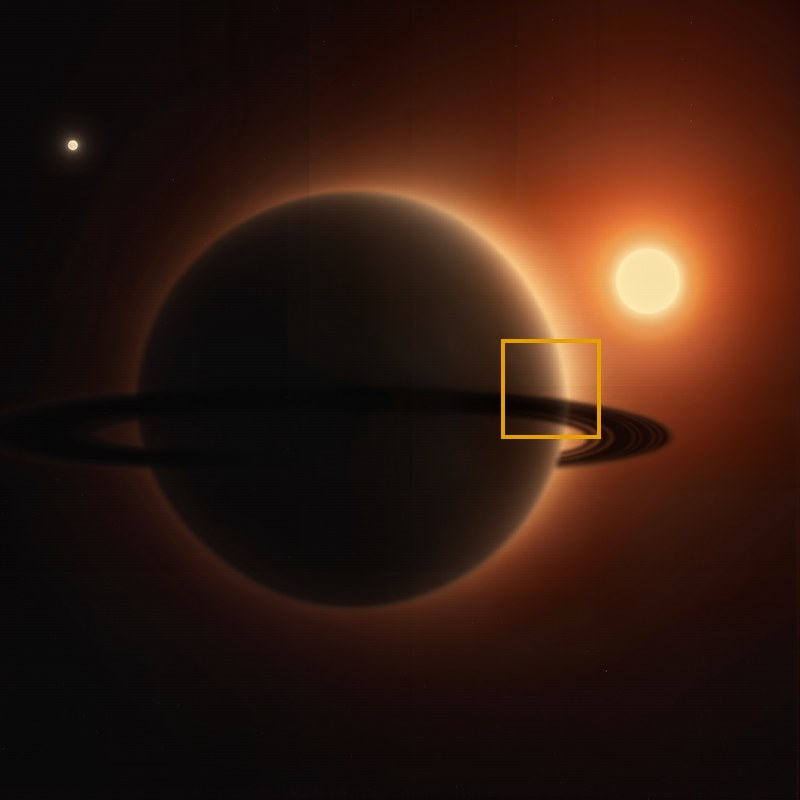
\includegraphics[height=0.1966\scaW]{figures/gallery_baselines/7961019668960160206_area.jpg}\hspace{0.0040\scaW}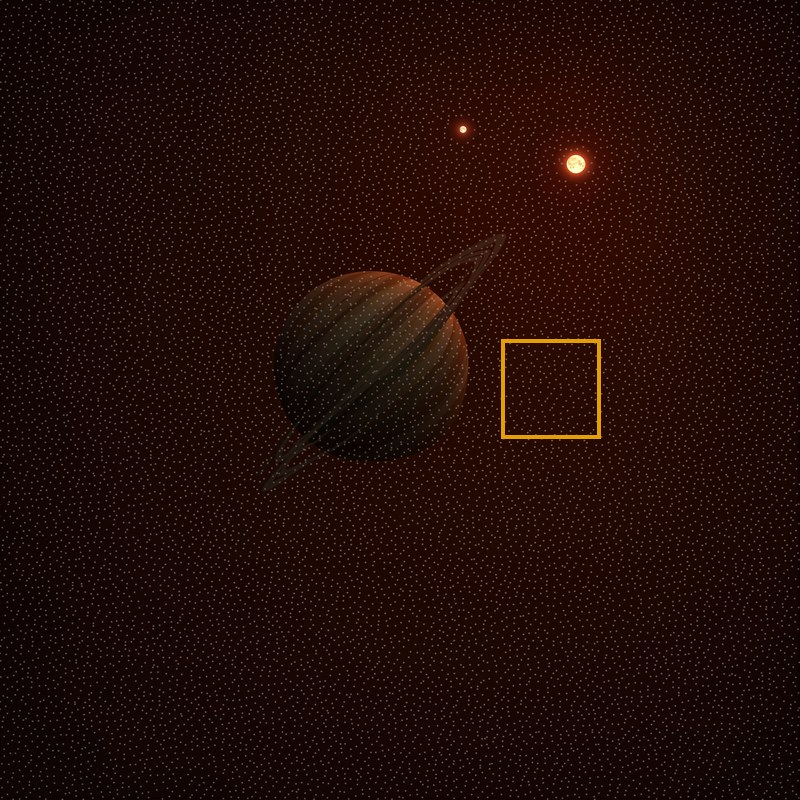
\includegraphics[height=0.1966\scaW]{figures/gallery_baselines/7961019668960160206_dype.jpg}\hspace{0.0040\scaW}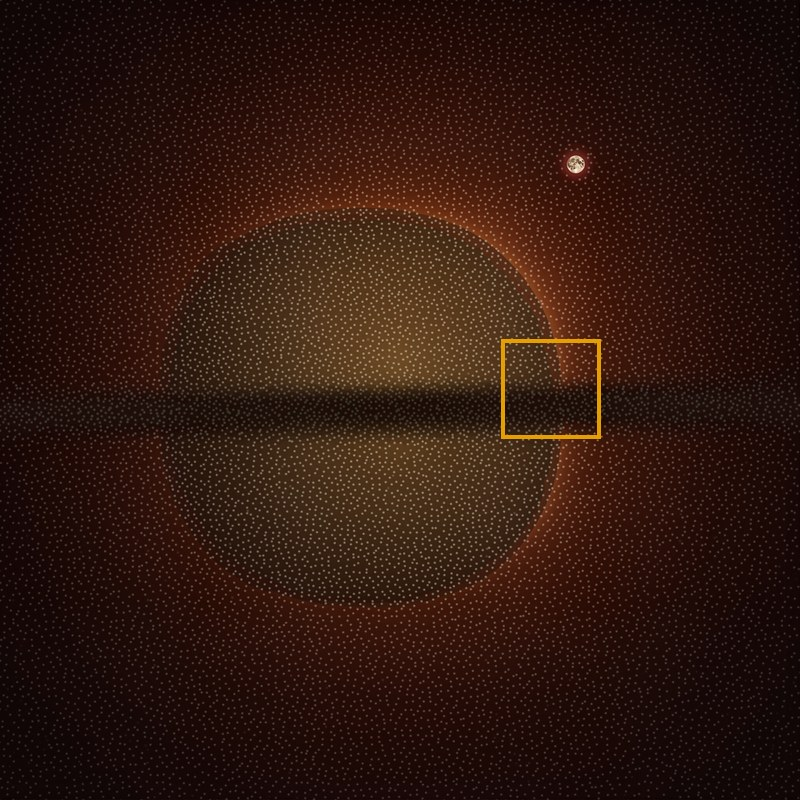
\includegraphics[height=0.1966\scaW]{figures/gallery_baselines/7961019668960160206_sega_official.jpg}\hspace{0.0040\scaW}
\includegraphics[height=0.1966\scaW]{figures/gallery_baselines/7961019668960160206_ultraimage.jpg}\hspace{0.0040\scaW}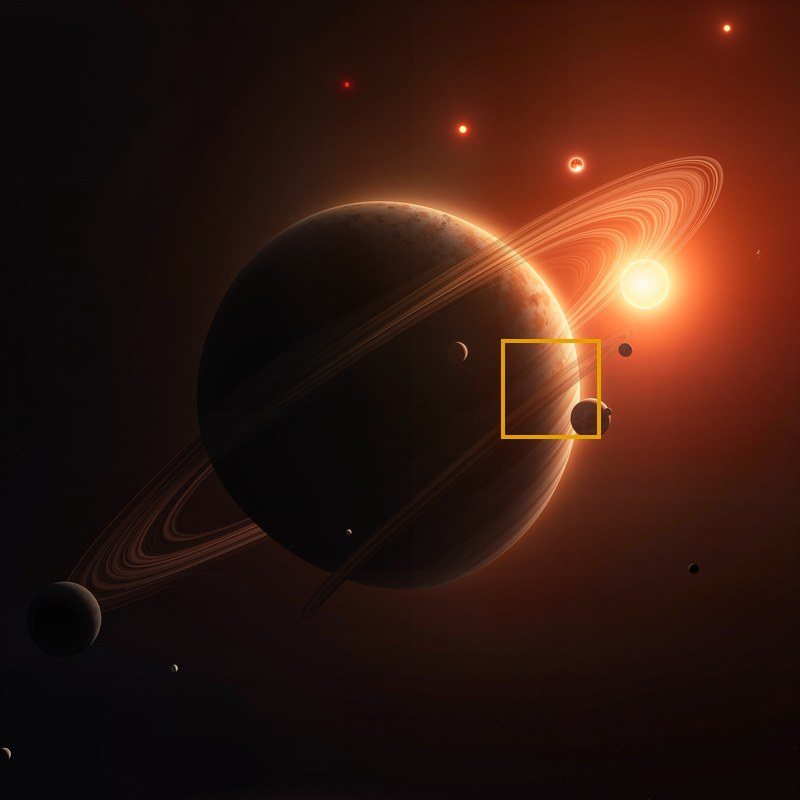
\includegraphics[height=0.1966\scaW]{figures/gallery_baselines/7961019668960160206_sca.jpg}}\\[0.0040\textwidth]
\makebox[\textwidth][l]{
\includegraphics[height=0.1966\scaW]{figures/gallery_baselines/7961019668960160206_area_crop.jpg}\hspace{0.0040\scaW}
\includegraphics[height=0.1966\scaW]{figures/gallery_baselines/7961019668960160206_dype_crop.jpg}\hspace{0.0040\scaW}
\includegraphics[height=0.1966\scaW]{figures/gallery_baselines/7961019668960160206_sega_official_crop.jpg}\hspace{0.0040\scaW}
\includegraphics[height=0.1966\scaW]{figures/gallery_baselines/7961019668960160206_ultraimage_crop.jpg}\hspace{0.0040\scaW}
\includegraphics[height=0.1966\scaW]{figures/gallery_baselines/7961019668960160206_sca_crop.jpg}}\\[0.0040\textwidth]
\makebox[\textwidth][l]{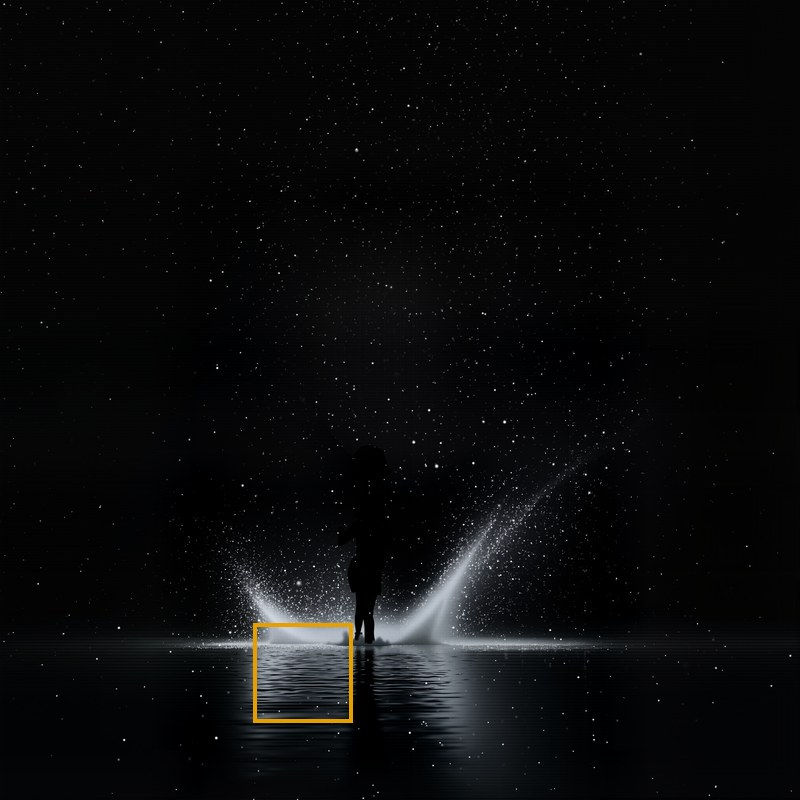
\includegraphics[height=0.1966\scaW]{figures/gallery_baselines/m2679953061215100202_area.jpg}\hspace{0.0040\scaW}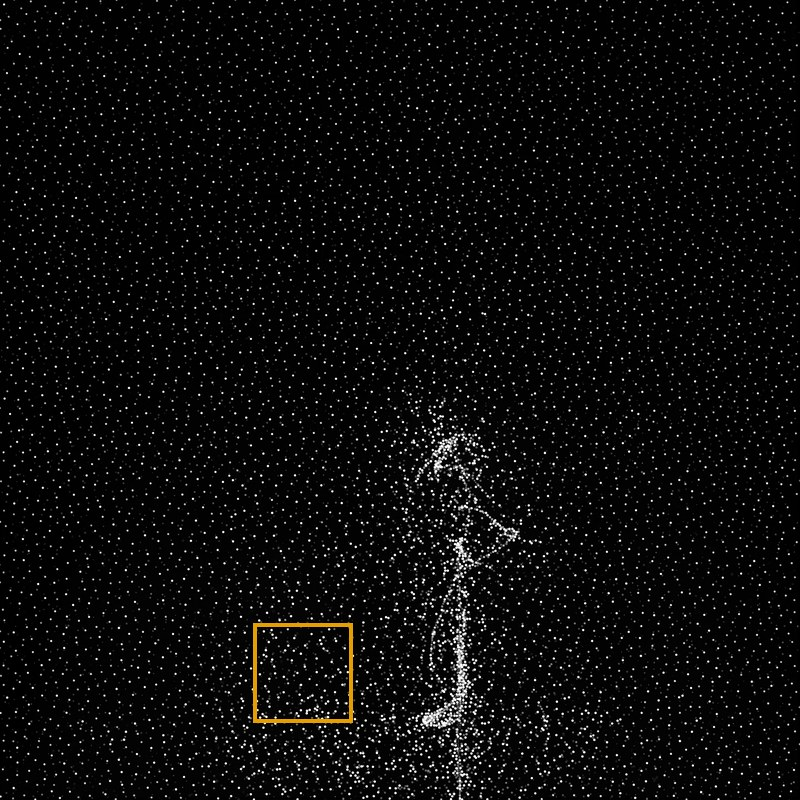
\includegraphics[height=0.1966\scaW]{figures/gallery_baselines/m2679953061215100202_dype.jpg}\hspace{0.0040\scaW}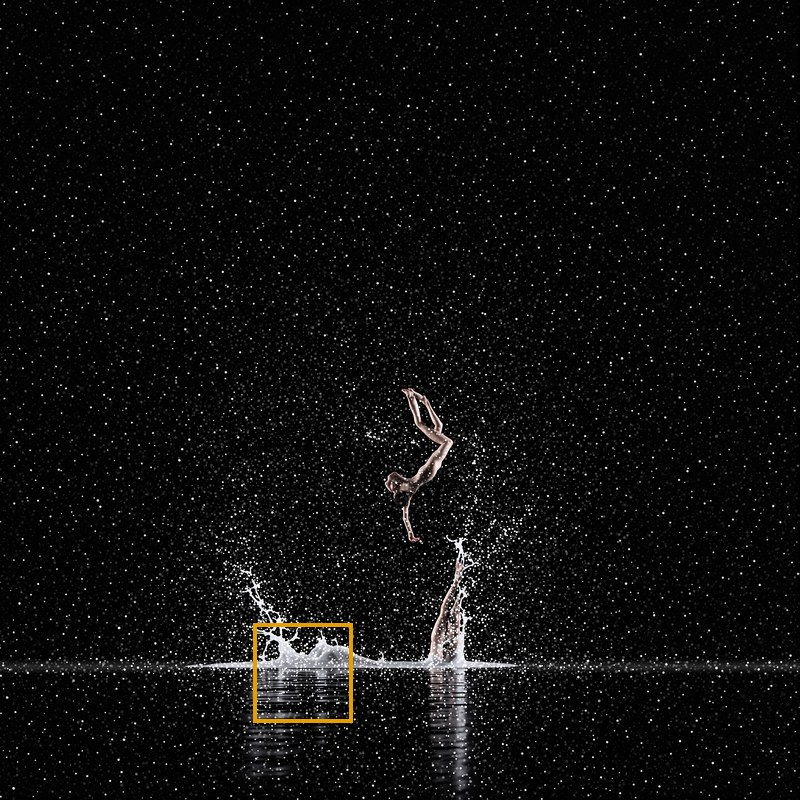
\includegraphics[height=0.1966\scaW]{figures/gallery_baselines/m2679953061215100202_sega_official.jpg}\hspace{0.0040\scaW}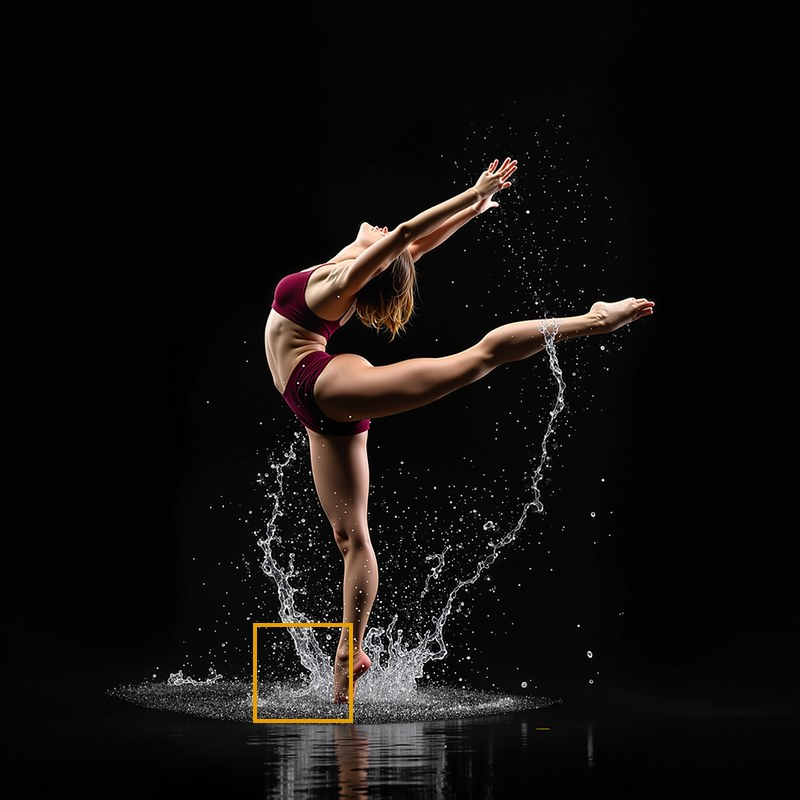
\includegraphics[height=0.1966\scaW]{figures/gallery_baselines/m2679953061215100202_ultraimage.jpg}\hspace{0.0040\scaW}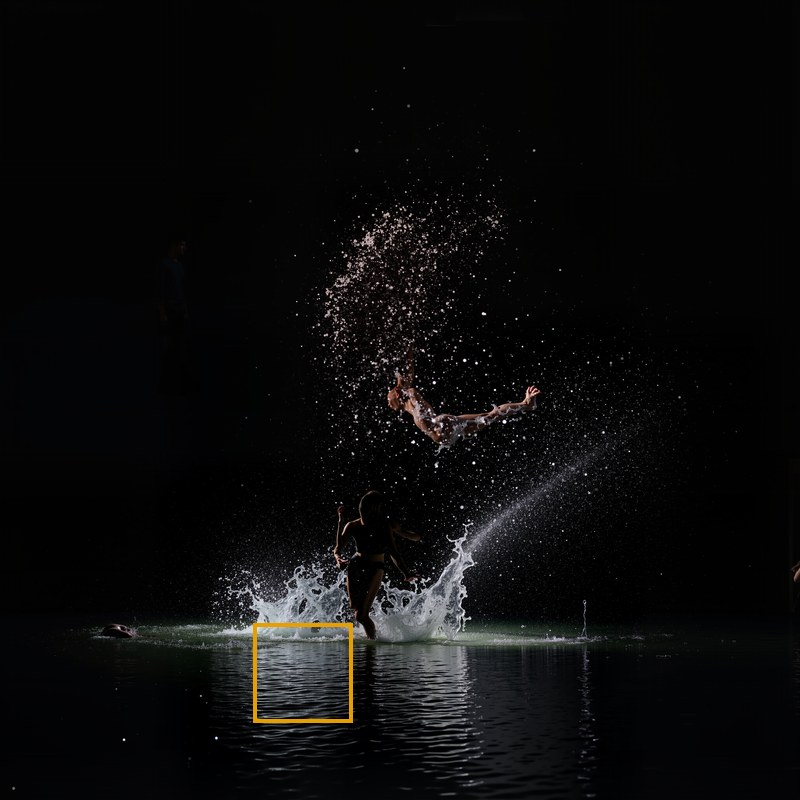
\includegraphics[height=0.1966\scaW]{figures/gallery_baselines/m2679953061215100202_sca.jpg}}\\[0.0040\textwidth]
\makebox[\textwidth][l]{
\includegraphics[height=0.1966\scaW]{figures/gallery_baselines/m2679953061215100202_area_crop.jpg}\hspace{0.0040\scaW}
\includegraphics[height=0.1966\scaW]{figures/gallery_baselines/m2679953061215100202_dype_crop.jpg}\hspace{0.0040\scaW}
\includegraphics[height=0.1966\scaW]{figures/gallery_baselines/m2679953061215100202_sega_official_crop.jpg}\hspace{0.0040\scaW}
\includegraphics[height=0.1966\scaW]{figures/gallery_baselines/m2679953061215100202_ultraimage_crop.jpg}\hspace{0.0040\scaW}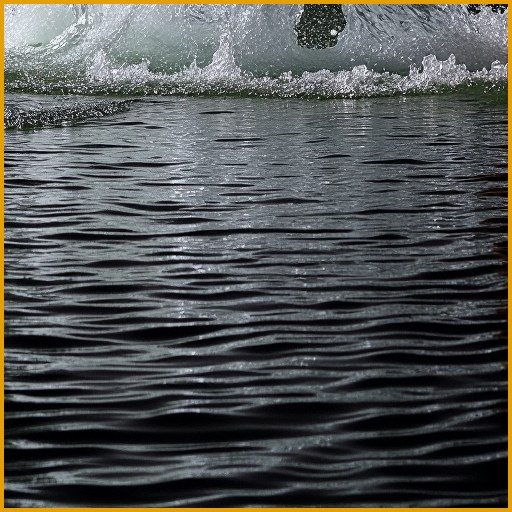
\includegraphics[height=0.1966\scaW]{figures/gallery_baselines/m2679953061215100202_sca_crop.jpg}}\\[0.0040\textwidth]
\makebox[\textwidth][l]{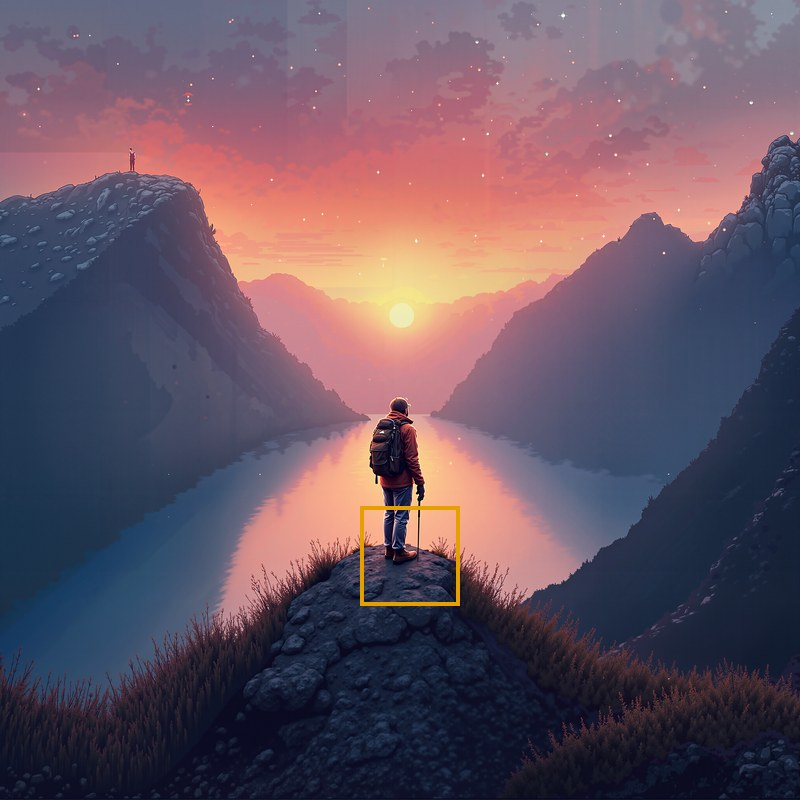
\includegraphics[height=0.1966\scaW]{figures/gallery_baselines/m4844341235185759356_area.jpg}\hspace{0.0040\scaW}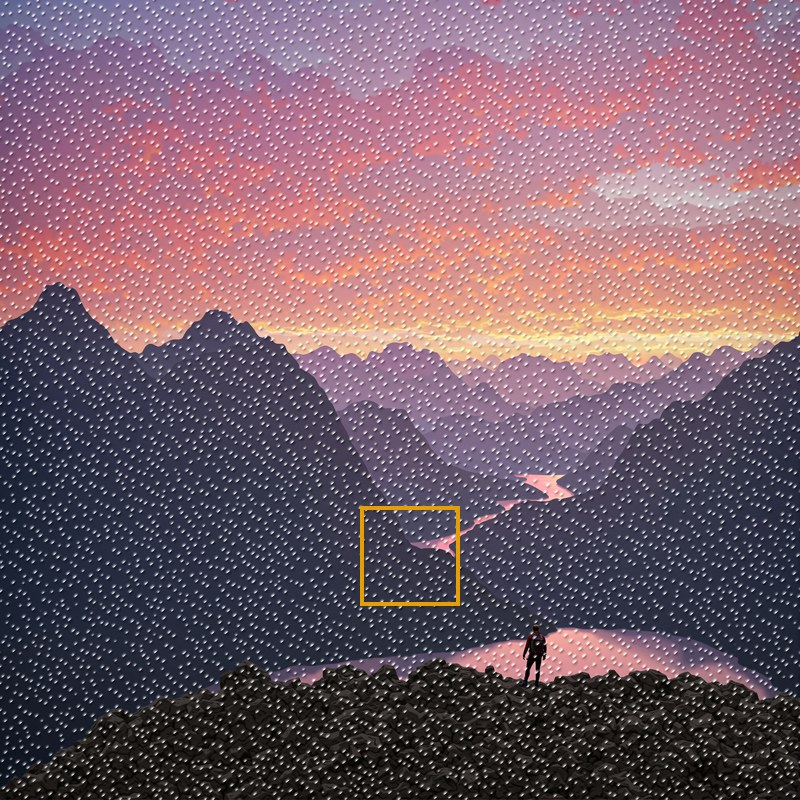
\includegraphics[height=0.1966\scaW]{figures/gallery_baselines/m4844341235185759356_dype.jpg}\hspace{0.0040\scaW}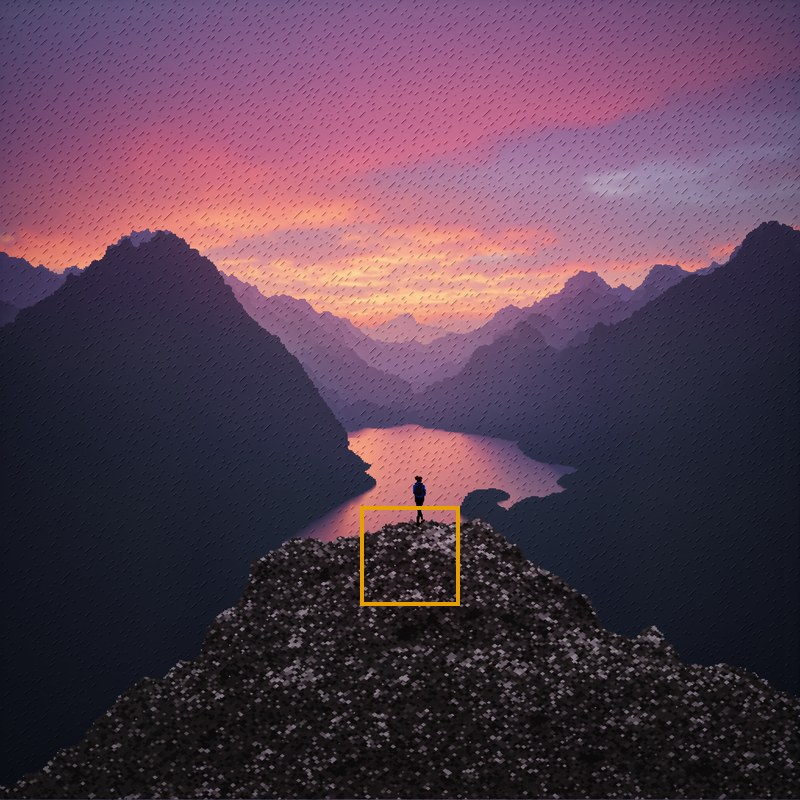
\includegraphics[height=0.1966\scaW]{figures/gallery_baselines/m4844341235185759356_sega_official.jpg}\hspace{0.0040\scaW}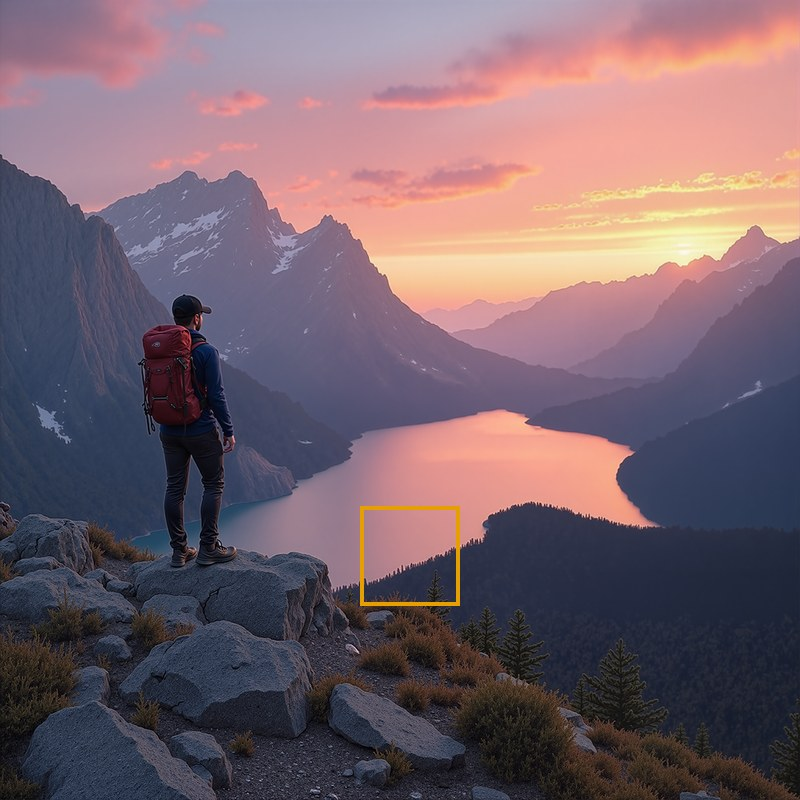
\includegraphics[height=0.1966\scaW]{figures/gallery_baselines/m4844341235185759356_ultraimage.jpg}\hspace{0.0040\scaW}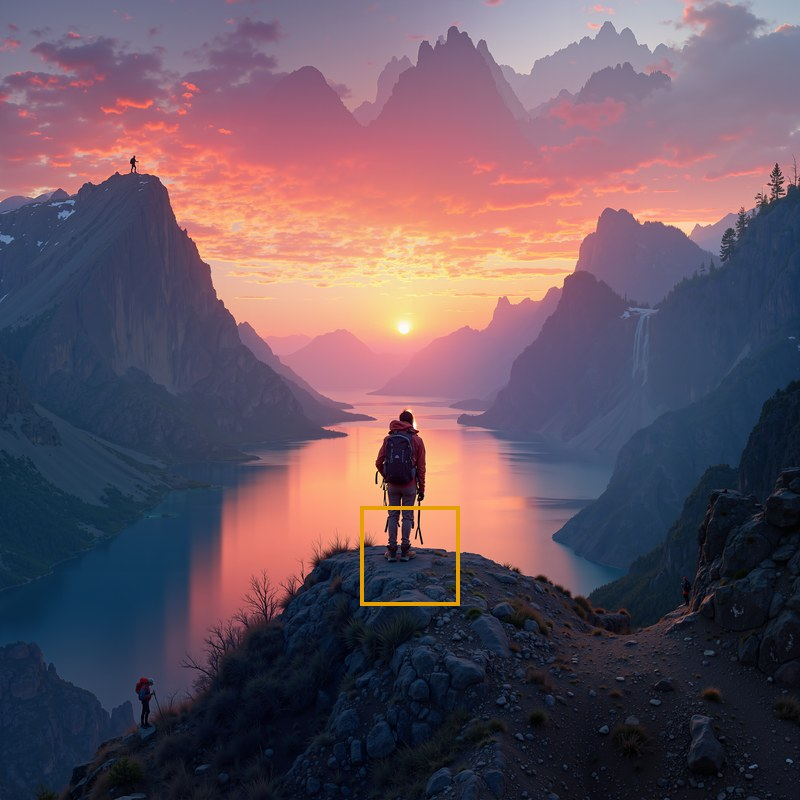
\includegraphics[height=0.1966\scaW]{figures/gallery_baselines/m4844341235185759356_sca.jpg}}\\[0.0040\textwidth]
\makebox[\textwidth][l]{
\includegraphics[height=0.1966\scaW]{figures/gallery_baselines/m4844341235185759356_area_crop.jpg}\hspace{0.0040\scaW}
\includegraphics[height=0.1966\scaW]{figures/gallery_baselines/m4844341235185759356_dype_crop.jpg}\hspace{0.0040\scaW}
\includegraphics[height=0.1966\scaW]{figures/gallery_baselines/m4844341235185759356_sega_official_crop.jpg}\hspace{0.0040\scaW}
\includegraphics[height=0.1966\scaW]{figures/gallery_baselines/m4844341235185759356_ultraimage_crop.jpg}\hspace{0.0040\scaW}
\includegraphics[height=0.1966\scaW]{figures/gallery_baselines/m4844341235185759356_sca_crop.jpg}}
\rmfamily\normalsize
\caption{\textbf{Additional baselines at $4096^2$.} Three randomly sampled paired prompts from the completed evaluation set, with no selection by visual quality or metric score. Each prompt occupies two rows: full images, then native-pixel crops of the outlined windows. FLUX.1-dev, seed 0. AReA, DyPE, SEGA and SCA use 28 steps and guidance 4.5; UltraImage uses its two-stage defaults (30+30 steps, guidance 3.5 then 7). The gallery illustrates outputs under these protocols, not equal-cost comparisons. Crop locations maximize edge energy averaged across the methods shown. Prompt selection uses seed 17; source hashes and crop coordinates are archived with the figure.}
\label{fig:gallery_baselines}
\end{figure*}
